\documentclass[11pt,journal,compsoc]{IEEEtran}

\ifCLASSOPTIONcompsoc
  \usepackage[nocompress]{cite}
\else
  \usepackage{cite}
\fi

\usepackage{graphicx}

\graphicspath{ {./images/}}

\DeclareGraphicsExtensions{.pdf,.jpeg,.png}

\usepackage{url}
\usepackage{xcolor}
\usepackage{subfig}
\usepackage{float}
\usepackage{url}
\usepackage{lipsum}
\def\UrlBreaks{\do\/\do-}
\usepackage{breakurl}
\usepackage[breaklinks]{hyperref}
\urlstyle{same}
\pagecolor{white}
\usepackage{alltt}
\usepackage[utf8x]{inputenc}
\DeclareUnicodeCharacter{2014}{\dash}
\usepackage{pifont}
\usepackage[toc,page]{appendix}
\usepackage{ragged2e}
\hypersetup{colorlinks=true,citecolor=blue,linkcolor=blue,urlcolor=blue,linktocpage=true}

\hyphenation{op-tical net-works semi-conduc-tor}

\linespread{1.0}
\begin{document}

\title{GET YOUR PERFECT FIT}

\author{Harsimran Kaur,~Karnik~Kalani,~Mounica~Ayalasomayajula,~Saumya~Sinha,~and~Vidushi~Bhati}

\IEEEtitleabstractindextext{%
\begin{abstract}
\testpar{Future of retail depends on giving customers the products which are best suited for them.There has been a surge in online shopping since the onset of the pandemic. Leading brands have been witnessing the increase in their online sales.People find online shopping more convenient and thus, online stores are keeping very limited stock in their stores rather than websites as people can buy several clothes from all the available or newly launched outfits by H \& M.Therefore, providing consumers with such an e-commerce platform that captures the wants of the customers has become imperative. This project aims to suggest the customer their best possible outfit according to their body shape.
Although, filters are available that provide customers outfits based on various parameters such as price, size, colour, and type. After evaluating the current H \& M Data-set, we came up with a plan to construct the architecture in such a way that customers can save their time by just providing a few details such as their age, size, body shape, colour preferences, skin tone, liking for specific fabrics while creating their accounts itself. Using these parameters users will be able to see only those outfits which will be best suited to them.
Also, will take into consideration if the customer is suffering from any textile related skin condition to suggest clothes made from suitable fabrics.It will also evaluate various other factors for gaining useful insights about the products.} \\
\\
\textbf{Keywords: H \& M, Data Analysis, SQL, Python, Cloud, AWS, JIRA, MySQL, MongoDB, Tableau, Jamboard, ETL, Spyder, Visual Studio}
 \\
Project GitHub: \href{https://github.com/DecipherData/data225semproj}{\textit{Link: https://github.com/DecipherData/data225semproj}} \\
\end{abstract}
}

\maketitle
\IEEEraisesectionheading{\section{Introduction}\label{sec:Introduction}}
Retail clothing industry has always been relevant and it continually strives to take all possible measures to gain a profitable edge in this highly competitive domain. Brands try to look at the granular level of what consumers want to retain their existing customers and attract the new ones. The interaction has increased directly or indirectly many folds with the advent of new technologies such as ML and AI. These technologies take into account the previous purchase patterns done by the customer and recommend clothes according to that. However, there is another aspect where a gap needs to be filled. Customer body shape and skin related conditions are not captured when customers register for some brand. Everybody is unique and not every style looks good on every body shape.Further, not all fabrics are suitable for everyone, So it is important for retailers to provide suggestions based on these factors.

\subsection{Motivation}\
\IEEEPARstart Fashion designers and stylists recommend their clients clothes that are a best fit for them based on their body shape and size. These skilled people are not accessible to everyone.The retailers only give suggestions to the customers based on their previous purchase patterns and sizes.If they were to give suggestions based on body types and further it by providing suggestions based on the skin conditions, many customers would save a lot of money and get their perfect fit. Also, customers may gain time by not spending time in trial rooms or if they have purchased an item online but was unsatisfactory after it arrived,then they need not waste time returning it.This will also benefit organizations who spend a considerable amount of money on logistics. Knowing the granular details of the customers may help brands in projecting what kind of clothes they need to stock up in their inventory and what kind they need to reduce manufacturing.

\subsection{Literature Survey}
To be able to provide suggestions according to the different body shapes, we must understand what types of body shapes exist. Idea of the body shapes are entirely subjective and arise from the societal standards that vary from culture to culture. \\
According to a study published in the International Journal of Clothing Science and Technology[1], There are seven types of female body shapes.It may be possible that some body shapes may not fit into the categories mentioned above.But for the scope of this project we are focusing on these seven body types. \\\\
\textbf{Body Types:}\\\\
\textbullet\textbf{Apple or Inverted Triangle:} \\
This body shape has relatively smaller hips than their shoulders and bust.
Range:  (bust – hips) ≥ 3.6″ AND (bust – waist) \textless \ 9″. \\\\
\textbullet\textbf{Banana, straight, or rectangle:} \\
This body shape has shoulders, waist, hip and busts  of similar size.The body is somewhat rectangular looking.
Range: (hips – bust) \textless \ 3.6″ AND (bust – hips) \textless \ 3.6″ AND (bust – waist) \textless \ 9″ AND 
(hips – waist) \textless \  10″. \\\\
\textbullet\textbf{Pear, spoon, bell, or triangle:} \\
This body shape has narrow bust and shoulders but has hips on the heavier side. With slender arms and shoulders,weight is distributed in the leg.
Range: If (hips – bust) \textgreater \  2″ AND (hips – waist) ≥ 7″ AND (high hip/waist) ≥ 1.193. \\\\
\textbullet\textbf{Hourglass, X shape, triangle, 
opposing,  or facing } \textbf{inwards:} \\
This body shape has nearly equal hips and bust with a relatively smaller well-defined waist.
Range:(bust – hips) ≤ 1″ AND (hips – bust) \textgreater \ 3.6″ AND (bust – waist) ≥ 9″ OR (hips – waist) ≥ 10″ \\\\
\textbullet\textbf{Top Hourglass:}\\
This body shape has hips smaller than bust and has a well-defined waist.
Range: (bust – hips) \textgreater \ 1″ AND (bust – hips) \textless \ 10″ AND (bust – waist) ≥ 9″ \\\\
\textbullet\textbf{Bottom Hourglass:} \\
This body shape is generally an hourglass shape but with hips slightly larger than bust.
 Range: (hips – bust) ≥ 3.6″ AND (hips – bust) \textless \ 10″ AND (hips – waist) ≥ 9″ AND (high hip/waist) \textless \ 1.193 \\\\
\textbullet\textbf{Fabrics:}\\
\ Clothing products are made of different materials.There are many people with sensitive skin or with other skin conditions such as eczema, dermatitis, Psoriasis. Cancer patients who go through radiations have sensitive skin and may develop rashes and sores from chemotherapy sessions.These patients if exposed to rough and bad quality fabric may aggravate their pain and discomfort.In our project we classify fabrics as good-for-skin (highest quality),medium quality and bad-for-sensitive-skin(low quality). \\\\
\textbullet\textbf{Good-for-skin(highest quality) fabric examples are:}\\ Silk, cotton, Linen, Flax, Hemp, Wool, cashmere, Crepe, Damask, Muslin, lace, satin, Chiffon, Organza. \\\\
\textbullet\textbf{Medium quality fabric examples are:}\\ Rayon, velvet, twill, acrylics, viscose, chenille\\\\
\textbullet\textbf{Low quality examples are:}\\
Spandex, polyester, nylon, leather, rubber, Tweed, Felt, 
Jute, Taffeta, Baize, Dyes, Anthraquinone \\\\
\textbullet\textbf{Skin conditions can be categorized into :}\\ 
1- severe, 2- medium and 3- no issues.
\subsection{Functional Requirements} 
A functional requirement defines an input required or dependency for us to complete our task. \\Following are the functional requirements of our project - Different attributes of data: customer, fabric, skin condition, product related. \\
A general perspective of available measurements are stereotyped and we want a bit of customization to be included in our body type declaration, for a customer to filter out product, based on many factors including fabric materials for their skin condition.
\subsection{Methodology}
We have collected data from different sources and also synthesized some data as per our functional requirements. \\
Once we drafted an initial version of our  ER-diagram using draw.io , we extracted the required data and cleaned the data using python in Visual studio code by dropping the columns that were no required, removing the duplicates, using NumPy to Clean Columns, and checking for the missing data and assigning values accordingly for the data to be ready. The respective tables were then created and data was inserted into them using MySQL Workbench to get practical perspective on data. MongoDB cluster was used for storing and accessing the body measurement configurations.\\
Python connection was established to MySQL server for developing few functions to implement logical decisions based on the SQL tables and data. \\
Once the modifications and operations are done on data and it is ready, AWS S3 was used to keep our contact and AWS Redshift cluster with database was created. AWS GLUE was also used to create and load our tables and data. Analysis was done in Redshift. Queries were formed to get insights about what fabric related sales were and how many different products contained what styles and fabrics, what products were there for different body type measurements etc. To introduce bit of customization to these products we tried to recognize the parameters that were top influential. AWS S3 buckets are correspondingly used by Redshift tables for storage, and used AWS Glue for performing ETL process.  \\
Tableau was used for displaying the result by connecting it with our AWS Redshift database. For all this work to be version controlled and to be properly coordinated,GIT was used.
\section{Project Walk-through}
\subsection{Data Sourcing and modeling} \\
\textbf{Data Sets:}\

\textbullet \textbf{Customer data:} \href{https://data.mendeley.com/datasets/bjv6c9pmp4/1}{ Body Measurements Data}\

\textbullet \textbf{H \& M Data:} \href{https://www.kaggle.com/datasets/odins0n/hm256x256}{ H \& M Data} \

\textbullet \textbf{Fabric data:} Synthesized by us from referring \ 

other links mentioned below in reference \ 

section.\\\\
\textbf{About the Data:} \

H \& M data includes products and transactions data that is in the public domain. It is de-normalized and is obfuscated for the purpose of publishing online. Considering the data as the initial set of data, we need to model ER diagrams and generate a normalized data model used by the brand. Since, we have a requirement of customer size specific data and fabric details of the product. This data is not present in the data-set. Therefore, we had to take 2-3 external data-sets and merge them to get different body measurements of customers and fabric types of products. Also, since our idea is novel based on different styles, such kind of data is not present so we had to look for different style types and generate the data according to our requirement. We have made the data models to address the following use cases which can be generalized for any brand in the market.
\newpage 
\noindent \textbf{Use Cases:} \\
Registration and login is out of scope.\\\\
\textbf{A. Customer}
\begin{itemize}
\item[\ding{220}]Assumption is that Customer has registered by providing relevant body measurements such as bust, hips, waist, high hip. 
\item[\ding{220}]Customer has given his/her skin condition level. 
\begin{itemize}
    \item Skin condition level 1 indicates: Severe skin conditions (eczema. psoriasis) 
    \item Skin condition level 2 indicates: Mild skin conditions (dryness, itchiness) 
    \item Skin condition level 3 indicates: No skin issues 
\end{itemize}
\item[\ding{220}]System should be able to evaluate the body type for each customer. 
\item[\ding{220}]Each body type may have one or more product styles associated with it. 
\end{itemize}
\textbf{B. Product available in online stores to its customers.}
\begin{itemize}
\item[\ding{220}]Each product is divided into three categories. 
\begin{itemize}
    \item Garment Upper Body 
    \item Garment Lower Body 
    \item Garment Full Body 
\end{itemize}
\item[\ding{220}]Each Product type is a part of one Product group. Product types can be Top, Blouse, Trouser, Skirt, Cardigan etc. (1-1) 
\item[\ding{220}]Each product can be of one product type. (1-1) 
\item[\ding{220}]Each product may have one or more colors associated with it. Also, each color may be associated with one or more products.(M-M) 
\item[\ding{220}]A product can be composed of multiple fabrics. Also, multiple products can be made from each fabric. (M-M) 
\item[\ding{220}]Each product may have one or more styles associated with it. Also, each style can be found in one or more products. (M-M) 
\item[\ding{220}]A style for a particular body should match the style associated with the product type. 
\item[\ding{220}]Each fabric should have a level indicating: 
\begin{itemize}
    \item Fabric level 1: Highest quality (skin-level 1 can wear these) 
    \item Fabric level 2: Medium quality (skin-level 2 can wear these + fabric level 1)
    \item Fabric level 3: Lowest quality (skin-level 3 can wear these + fabric level 1 + fabric level 2)
\end{itemize}
\end{itemize}

\begin{figure}
    \subsection{ER diagram}
    \subsubsection{Initial ER Diagram:}
    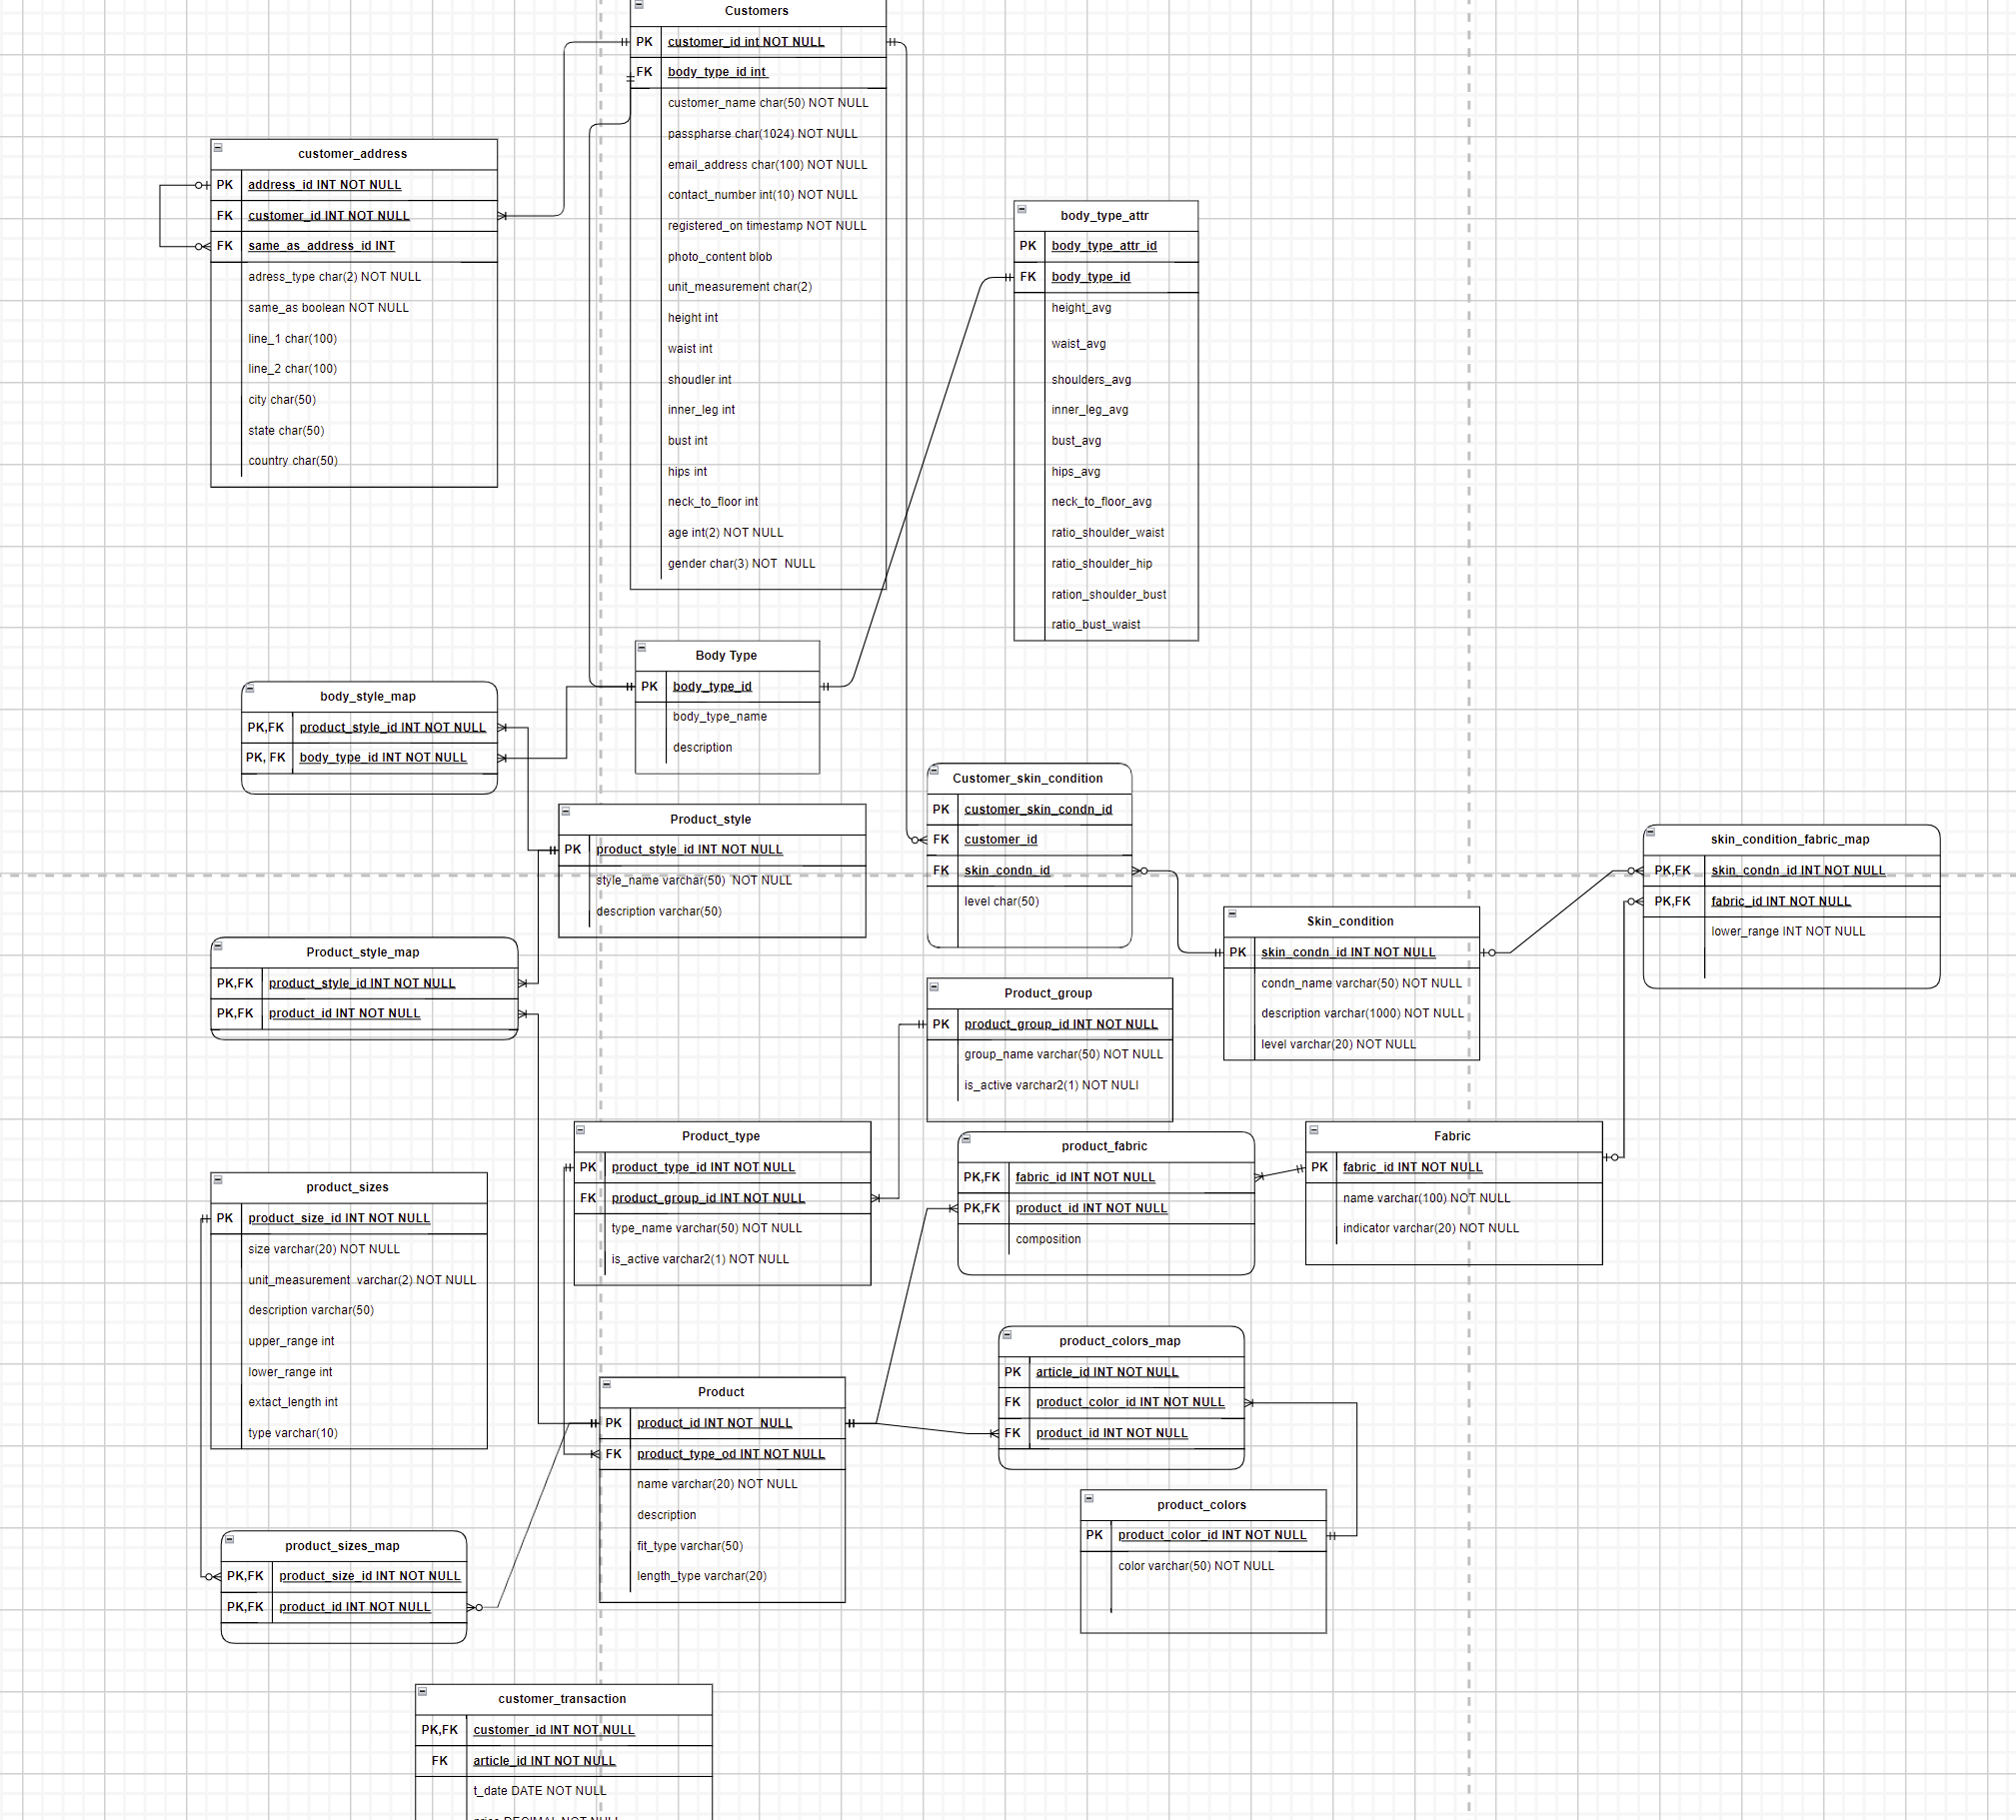
\includegraphics[scale=0.375]{images/ERDiagram.png}
    \caption{\href{https://www.kaggle.com/datasets/odins0n/hm256x256}{ Initial ER Diagram}}
    \subsubsection{Modified ER Diagram:} 
    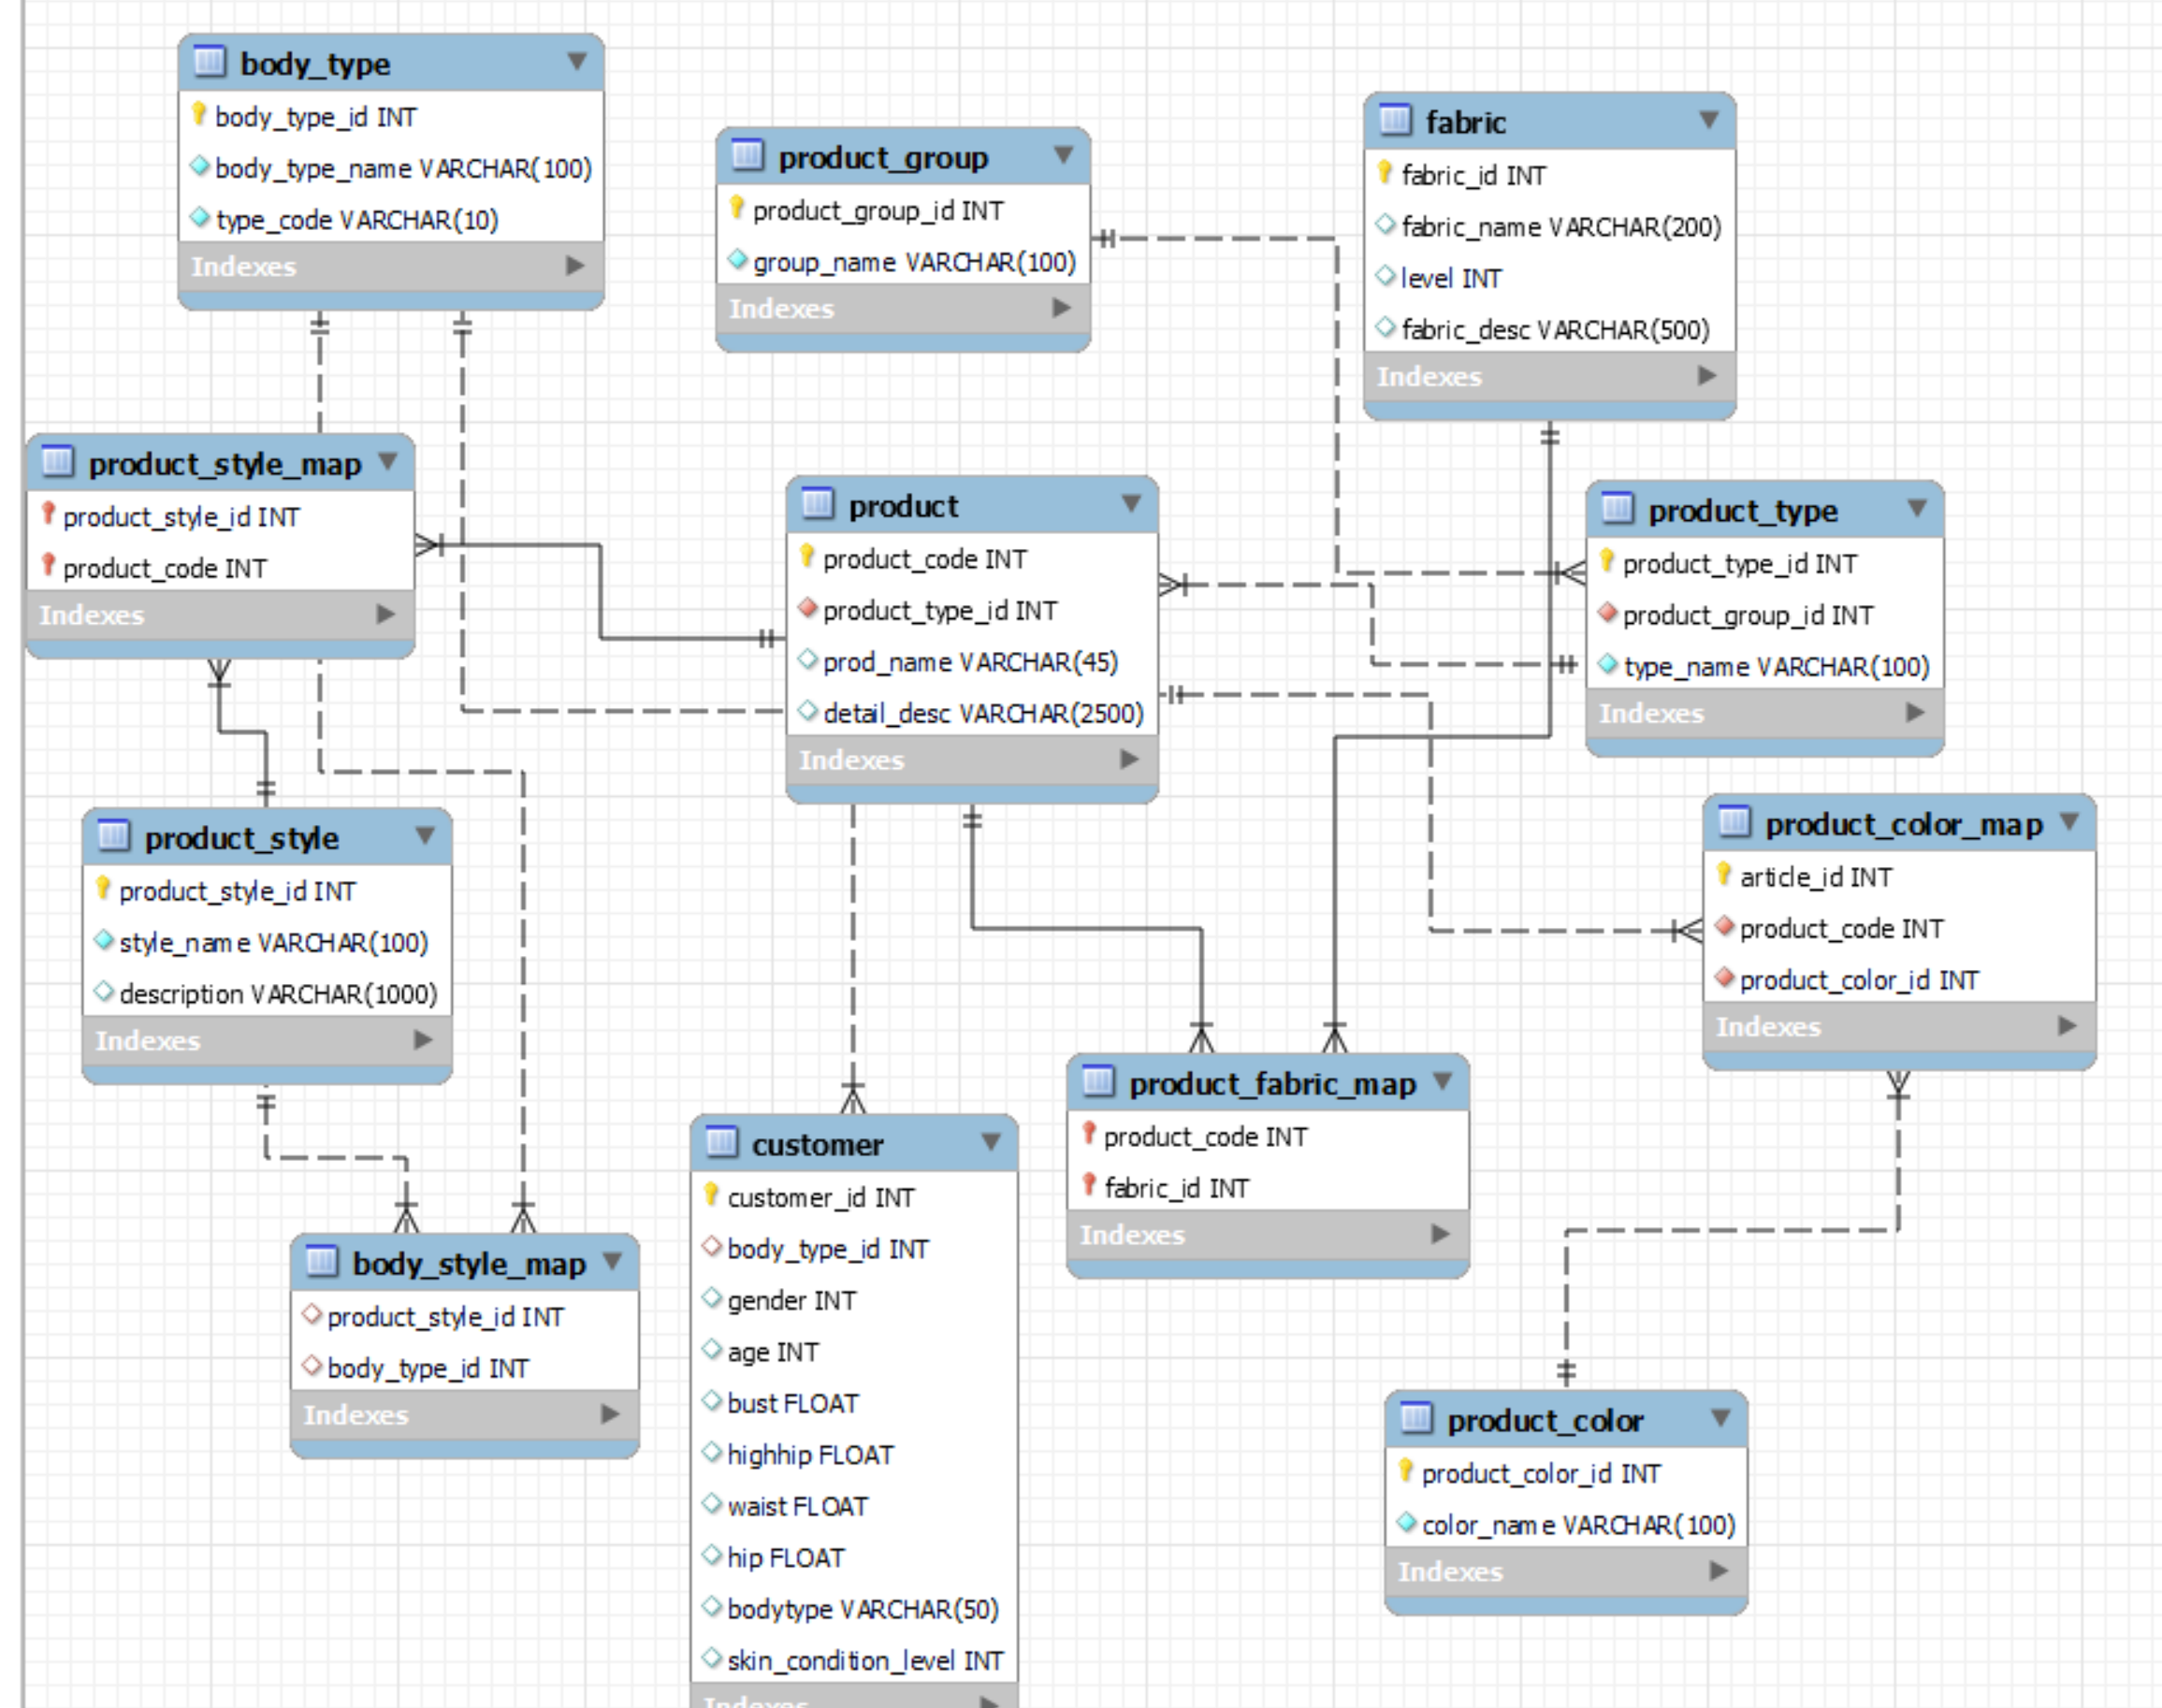
\includegraphics[scale=0.35]{images/ERdiagram_2.png}
    \caption{\href{https://www.kaggle.com/datasets/odins0n/hm256x256}{ Modified ER Diagram}}
    \subsubsection{Workflow Model:} 
    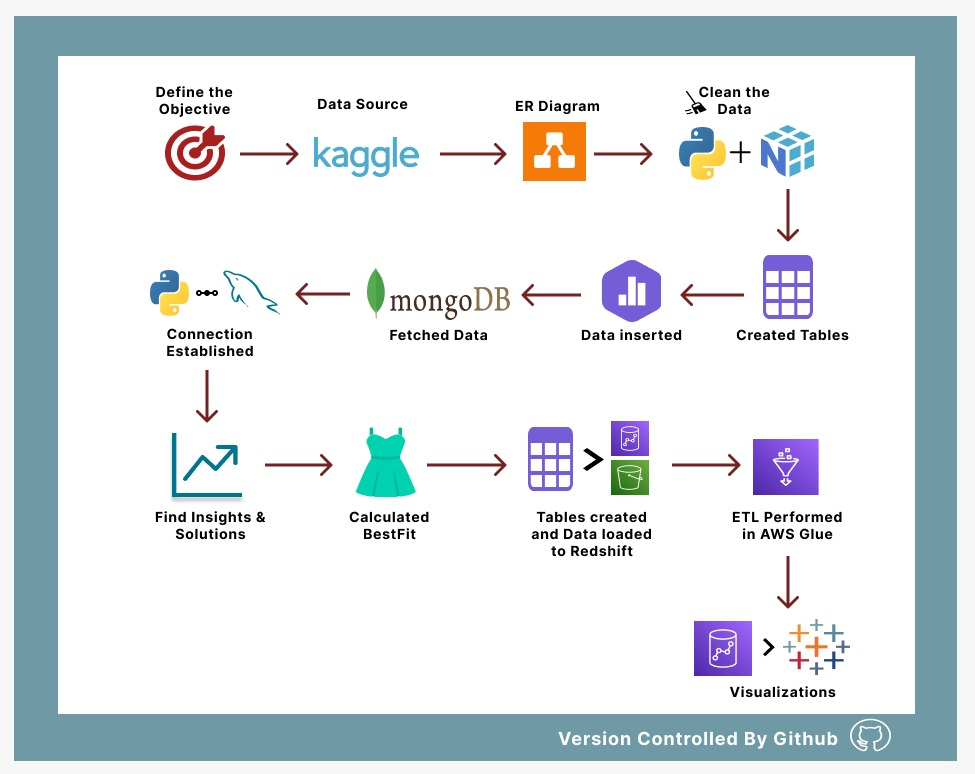
\includegraphics[scale=0.23]{images/workflow_hs.jpeg}
    \caption{\href{https://www.kaggle.com/datasets/odins0n/hm256x256}{ Workflow}}
\end{figure}

\subsection{Implementation} 
\begin{itemize}
    \item[\ding{220}] \textbf{Use of MS-Excel for new data:} Data is gathered from various sources and also some new data about product styles which is unique to our problem was taken from websites and was generated using Excel sheets. Use of Vlookup,IF statement and String concatenations were done for generating insertion queries for this new data that mapped product styles with body shapes.Columns denote body type and rows denote product style. “Y” denotes which style is suited for which body. If any cell is Y, then insertion queries were generated which were used for populating database tables.\\
    \item[\ding{220}] \textbf{Database connection/API connectivity:} Data is gathered from various sources and also some new data about product styles which is unique to our problem was taken from websites and was generated using Excel sheets. Use of Vlookup,IF statement and String concatenations were done for generating insertion queries for this new data that mapped product styles with body shapes.Columns denote body type and rows denote product style. “Y” denotes which style is suited for which body. If any cell is Y, then insertion queries were generated which were used for populating database tables.\\
    \item[\ding{220}] \textbf{Connection with MYSQL workbench:} The configuration file for connecting with databases is added so that different sections for different databases can be made and utilized for connecting to different data sources.The configuration parser API parses the file using which connection to MySQL server is made.\\
    \item[\ding{220}] \textbf{Connection with MongoDB cluster:} Standalone MongoDB cluster is made that is running in the containerized docker instance. Database ProjectData225 is created with bodytype as collection. Standard body measurements parameters for each body type are kept here for referencing  purposes later when they would be used for calculation of body shapes of the customers.\\
    \item[\ding{220}] \textbf{Other data in the form of CSVs were extracted, cleaned and loaded using Python:} Since our main CSV file has so many columns which may be relevant to 'H \& M' but irrelevant to our problem hence, columns such as graphical color related, perceived related and index related were dropped. In our project, we are taking into account just three categories; Garment Lower body, Garment Upper Body and Garment Full body. Rest all the rows of product groups were dropped. There were places where columns had null values that were replaced by None in the description of the product.\\
    \item[\ding{220}] \textbf{Several Main Tables and junction tabled were populated using python:} Static data about product style,fabric, bodytype and other tables are inserted using scripts and python code. Other tables such as product, Productcolormap, Fabriccolormap etc are inserted after looking for which style and fabric is associated with which product by parsing a detail description column in the main article file.\\
    \item[\ding{220}] \textbf{Several Main Tables and junction tabled were populated using python:} Static data about product style,fabric, bodytype and other tables are inserted using scripts and python code. Other tables such as product, Productcolormap, Fabriccolormap etc are inserted after looking for which style and fabric is associated with which product by parsing a detail description column in the main article file.
\end{itemize}

\subsection{Python code} \

Since our main article csv file does not have granular details about the product styles as it is de-normalized.The general details about the product is given in the description column. So, we searched every product’s description using regular expression to find if the product has any style associated with it.If there was any style associated with the product,then its product code was captured that was then used by other tables for making connections of product styles with body type and product.Similarly, since fabric composition was not given in our main article file, We populated fabric related to a particular product by searching product name and description of each row using regular expression to find which fabric is associated with which product.This is essential because fabric is associated with skin condition level of the customer who wants to buy a product.
\begin{itemize}
    \item[\ding{118}] \textbf{Finding the body shape of the customer:}{ The customer measurements are taken and calculations are done using standard configuration taken from the MongoDB document. A customer will ideally fall into these seven categories of body shapes, if not then default is kept as hourglass.}
    \item[\ding{118}] \textbf{Creating Queries to find the perfect fit for the customer:}{ This can be done by supplying the program with customer id (such as  44, 85, 40, 42, 183), the product type the customer is looking for(such as Top, Trousers, Skirt, Cardigan, Jacket) and skin conditions, if any( 1- severe, 2-mild, 3-no issues). The program first calculates the body shape of the customer and then fetches the list of Product types with the fabric quality according to their skin condition level. Or if customer id is not available, Body shape can be given(such as rectangle,round,hourglass) along with product type and skin condition level to find the best possible outfit.}
\end{itemize}
\subsection{ETL}
\textbf{Steps Followed in AWS Redshift and AWS S3:}
\begin{itemize}
    \item[-] Store the CSV files in S3 Bucket.
    \item[-] Partitions are the folders in the S3 bucket.
    \item[-] Created cluster with name data225-group6.
    \item[-] Created tables in the database.
    \item[-] Stored the csv file records to the database tables using Load Data UI located in the Query editor v2 or use “Copy” command.
    \item[-] Using Load Data button UI in Query Editor which gives the “copy” command.
\end{itemize}
\textbf{Steps followed in AWS Glue:}
\newline For ETL, we have used AWS glue. For which we have created a database and tables (using crawler) for the same. Jobs were created and provided a source folder of S3.
\begin{itemize}
    \item[-] Created a database in AWS glue.
    \item[-] Added the tables using crawler from S3 bucket. 
    \item[-] Given crawler a name.
    \item[-] Selected Data Store as S3 and Choose your file from S3 Bucket path.
    \item[-] Selected the crawl data to be selected from existing account or another account.
    \item[-] Selected the IAM role which has the policy access required for AWS Glue.
    \item[-] We have selected frequency as “Run on demand” but hourly, monthly, weekly can also be selected.
\end{itemize}
\textbf{Final Review:}
\begin{itemize}
    \item[-] Crawler created successfully and executed.
    \item[-] Table successfully created by crawler.
    \item[-] Table schema and details after creation.
    \item[-] Created a Connection to keep the credentials saved in case required. 
\end{itemize}
\textbf{Created a job for ETL:}
\begin{itemize}
    \raggedright \item[-] Alter the Schema of the table if required.
    \item[-] Job is ready, we can alter the script accordingly and can also alter the file format before running the job.
    \item[-] Table schema and details after creation.
    \item[-] After running the job. Following files have been created and if records are more, the job separated one csv file into multiple csv files.
\end{itemize}
\textbf{Same Process is repeated for transactions.csv file.}
\section{Data Analysis and Visualization}
\subsection{Insights according to our proposal} 
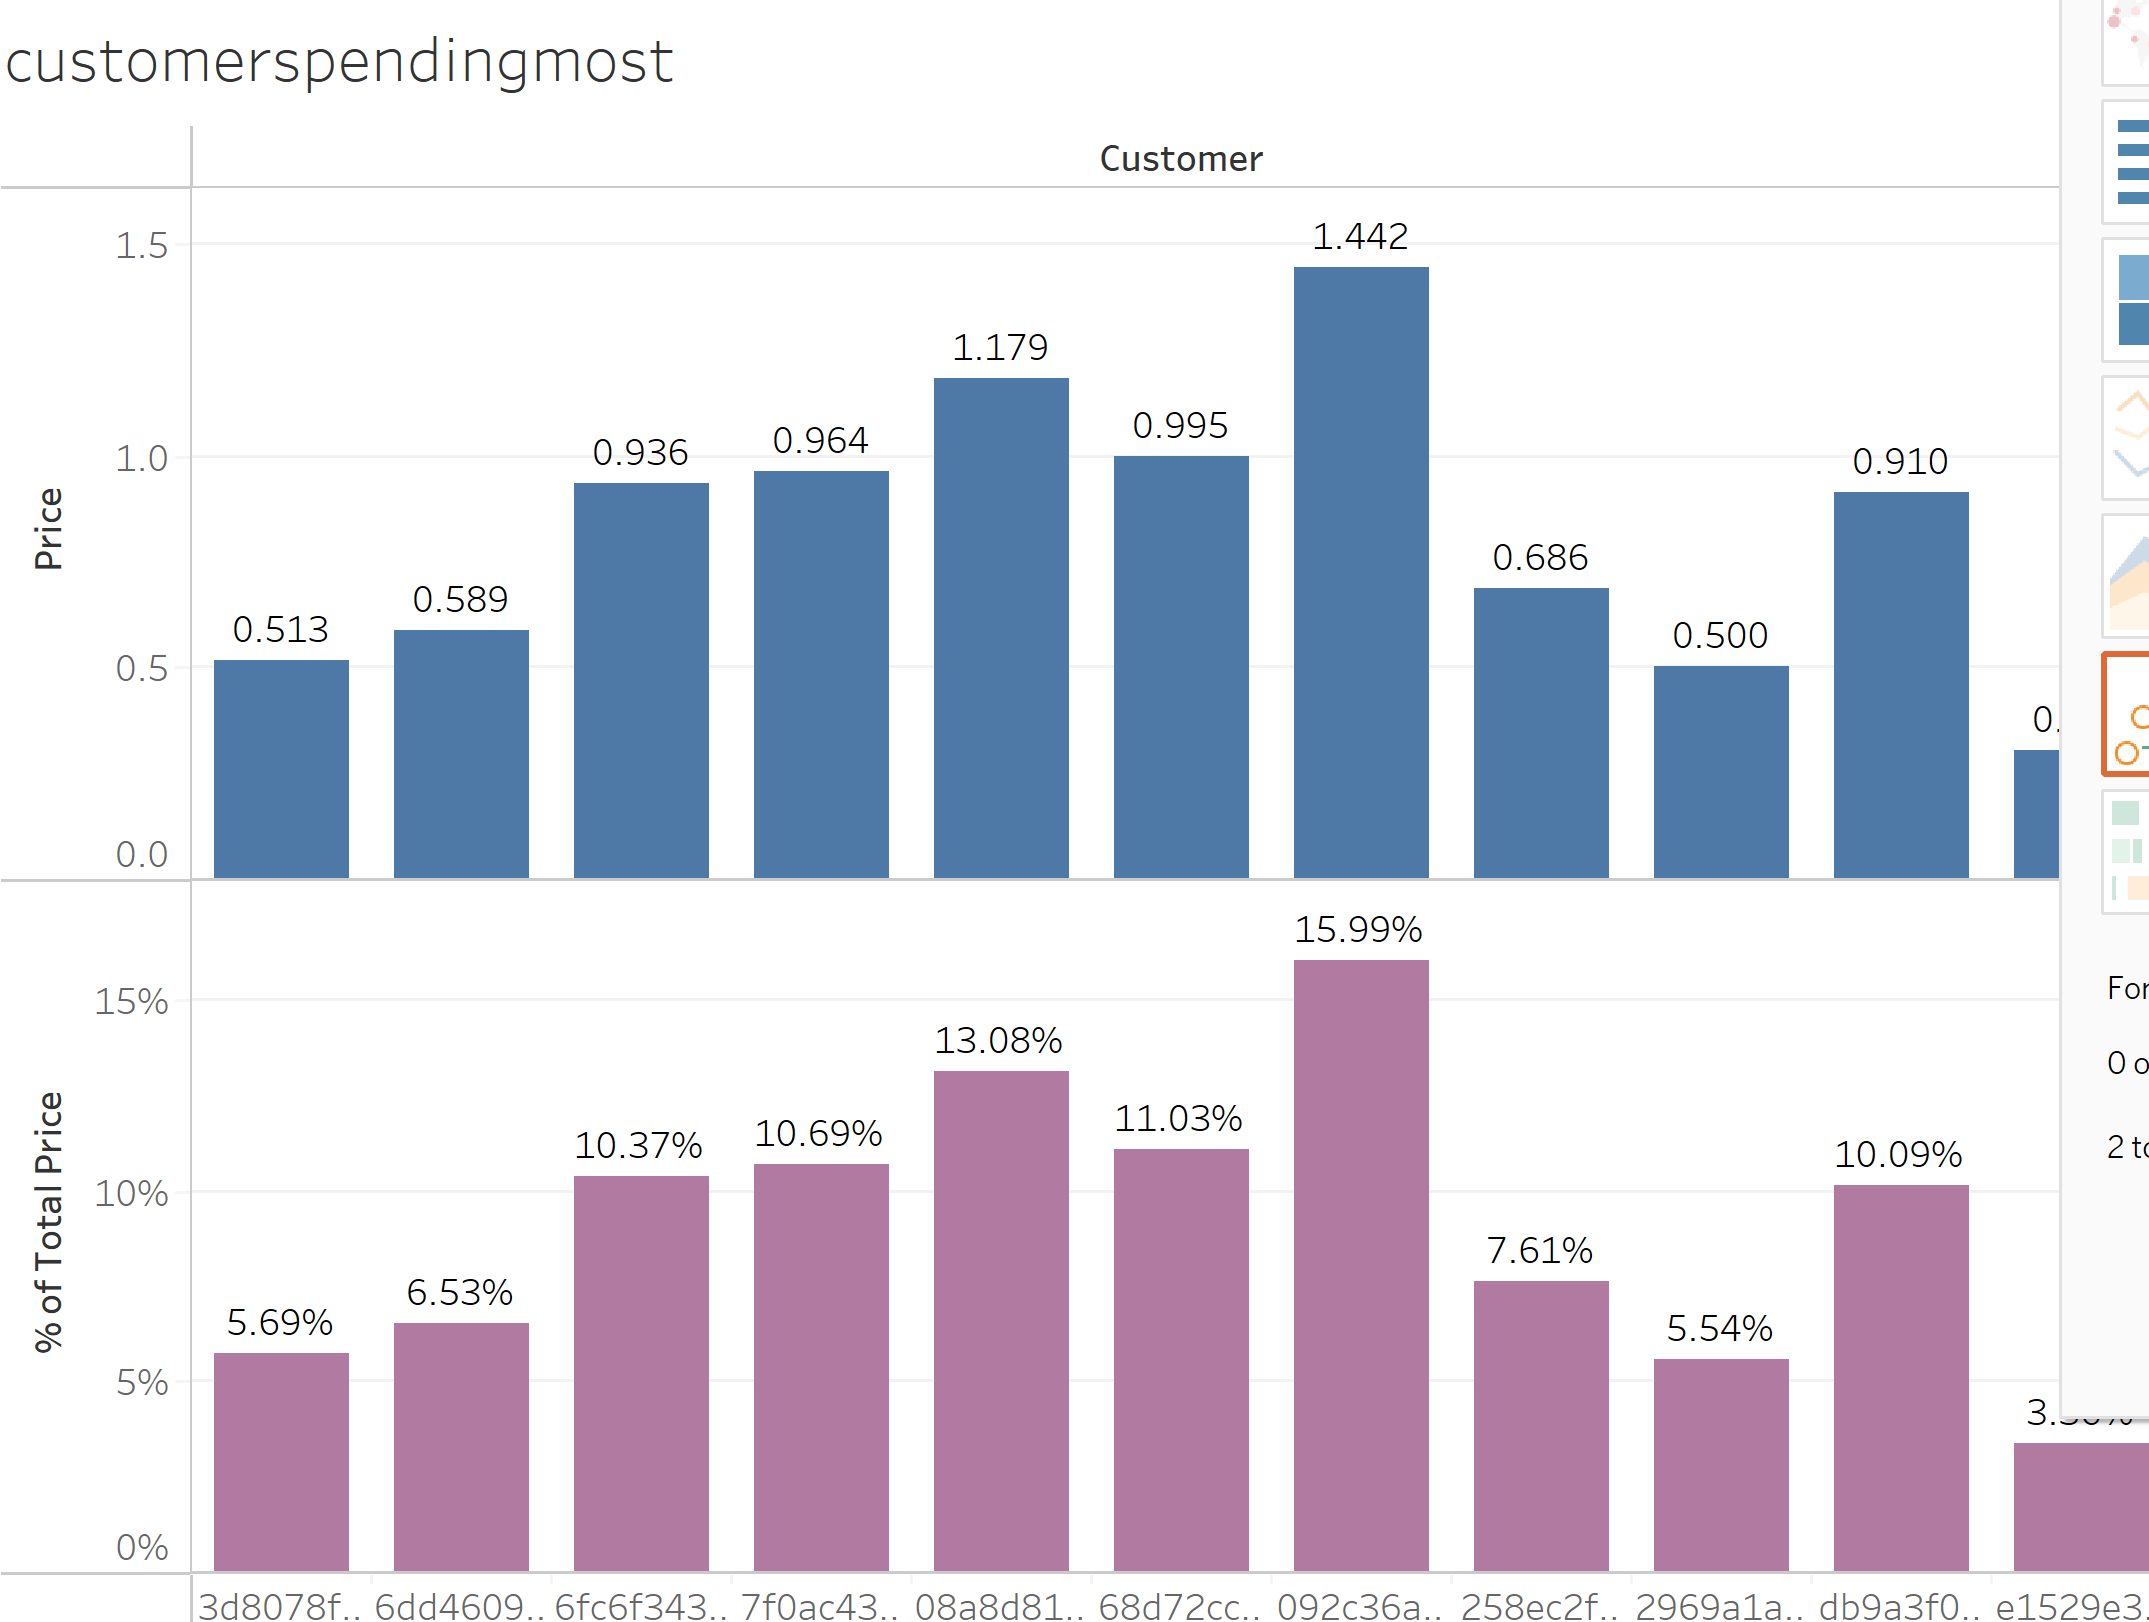
\includegraphics[scale=0.35]{images/customer.png} 
\newline \centering{{\href{https://github.com/DecipherData/data225semproj/blob/main/Screenshots/customer.png}{Figure 4}}}\\
\justifying These are the list of the customers that has spend most amount of money on the purchase of items.The prices in the original data-set are scaled down between 0 and 1.This is a useful insight to know which customers have more spending power and teams may use different strategies to retain these customers.Also, provide incentives such as coupons, promotion codes to low spending customers to attract more sales.\

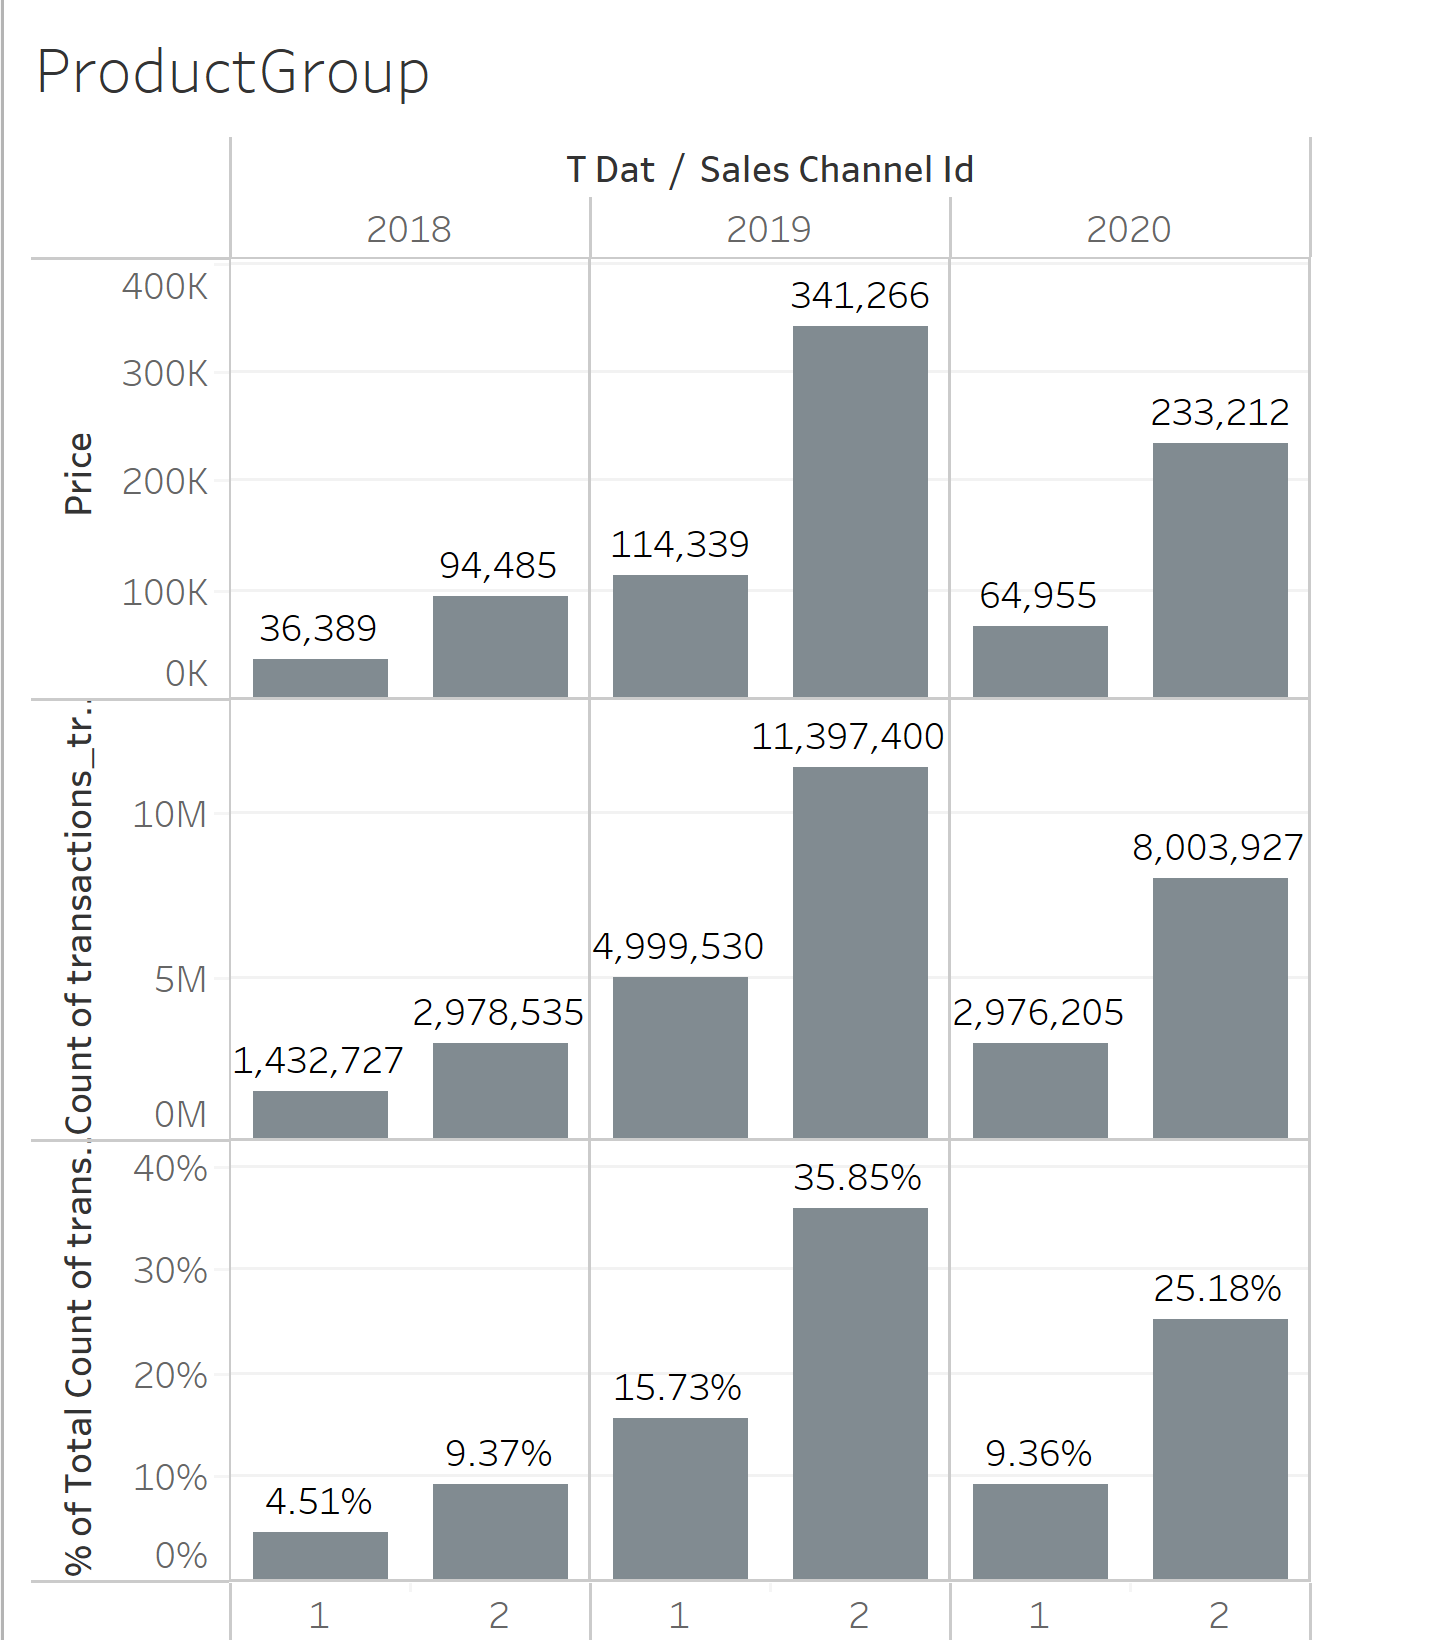
\includegraphics[scale=0.35]{images/date.png}
\newline \centering{{\href{https://github.com/DecipherData/data225semproj/blob/main/Screenshots/date.png}{Figure 5}}}\\
\justifying The above figure shows the distribution of transactions between two sales channels across the years, 2018-2020.We do not have full yearly data for 2018.so, we will not analyze this year.Comparing between 2019 and 2020, sales were significantly dropped in both the channels.This may be due to the  effect of pandemic on stores getting closed and people spending less.\

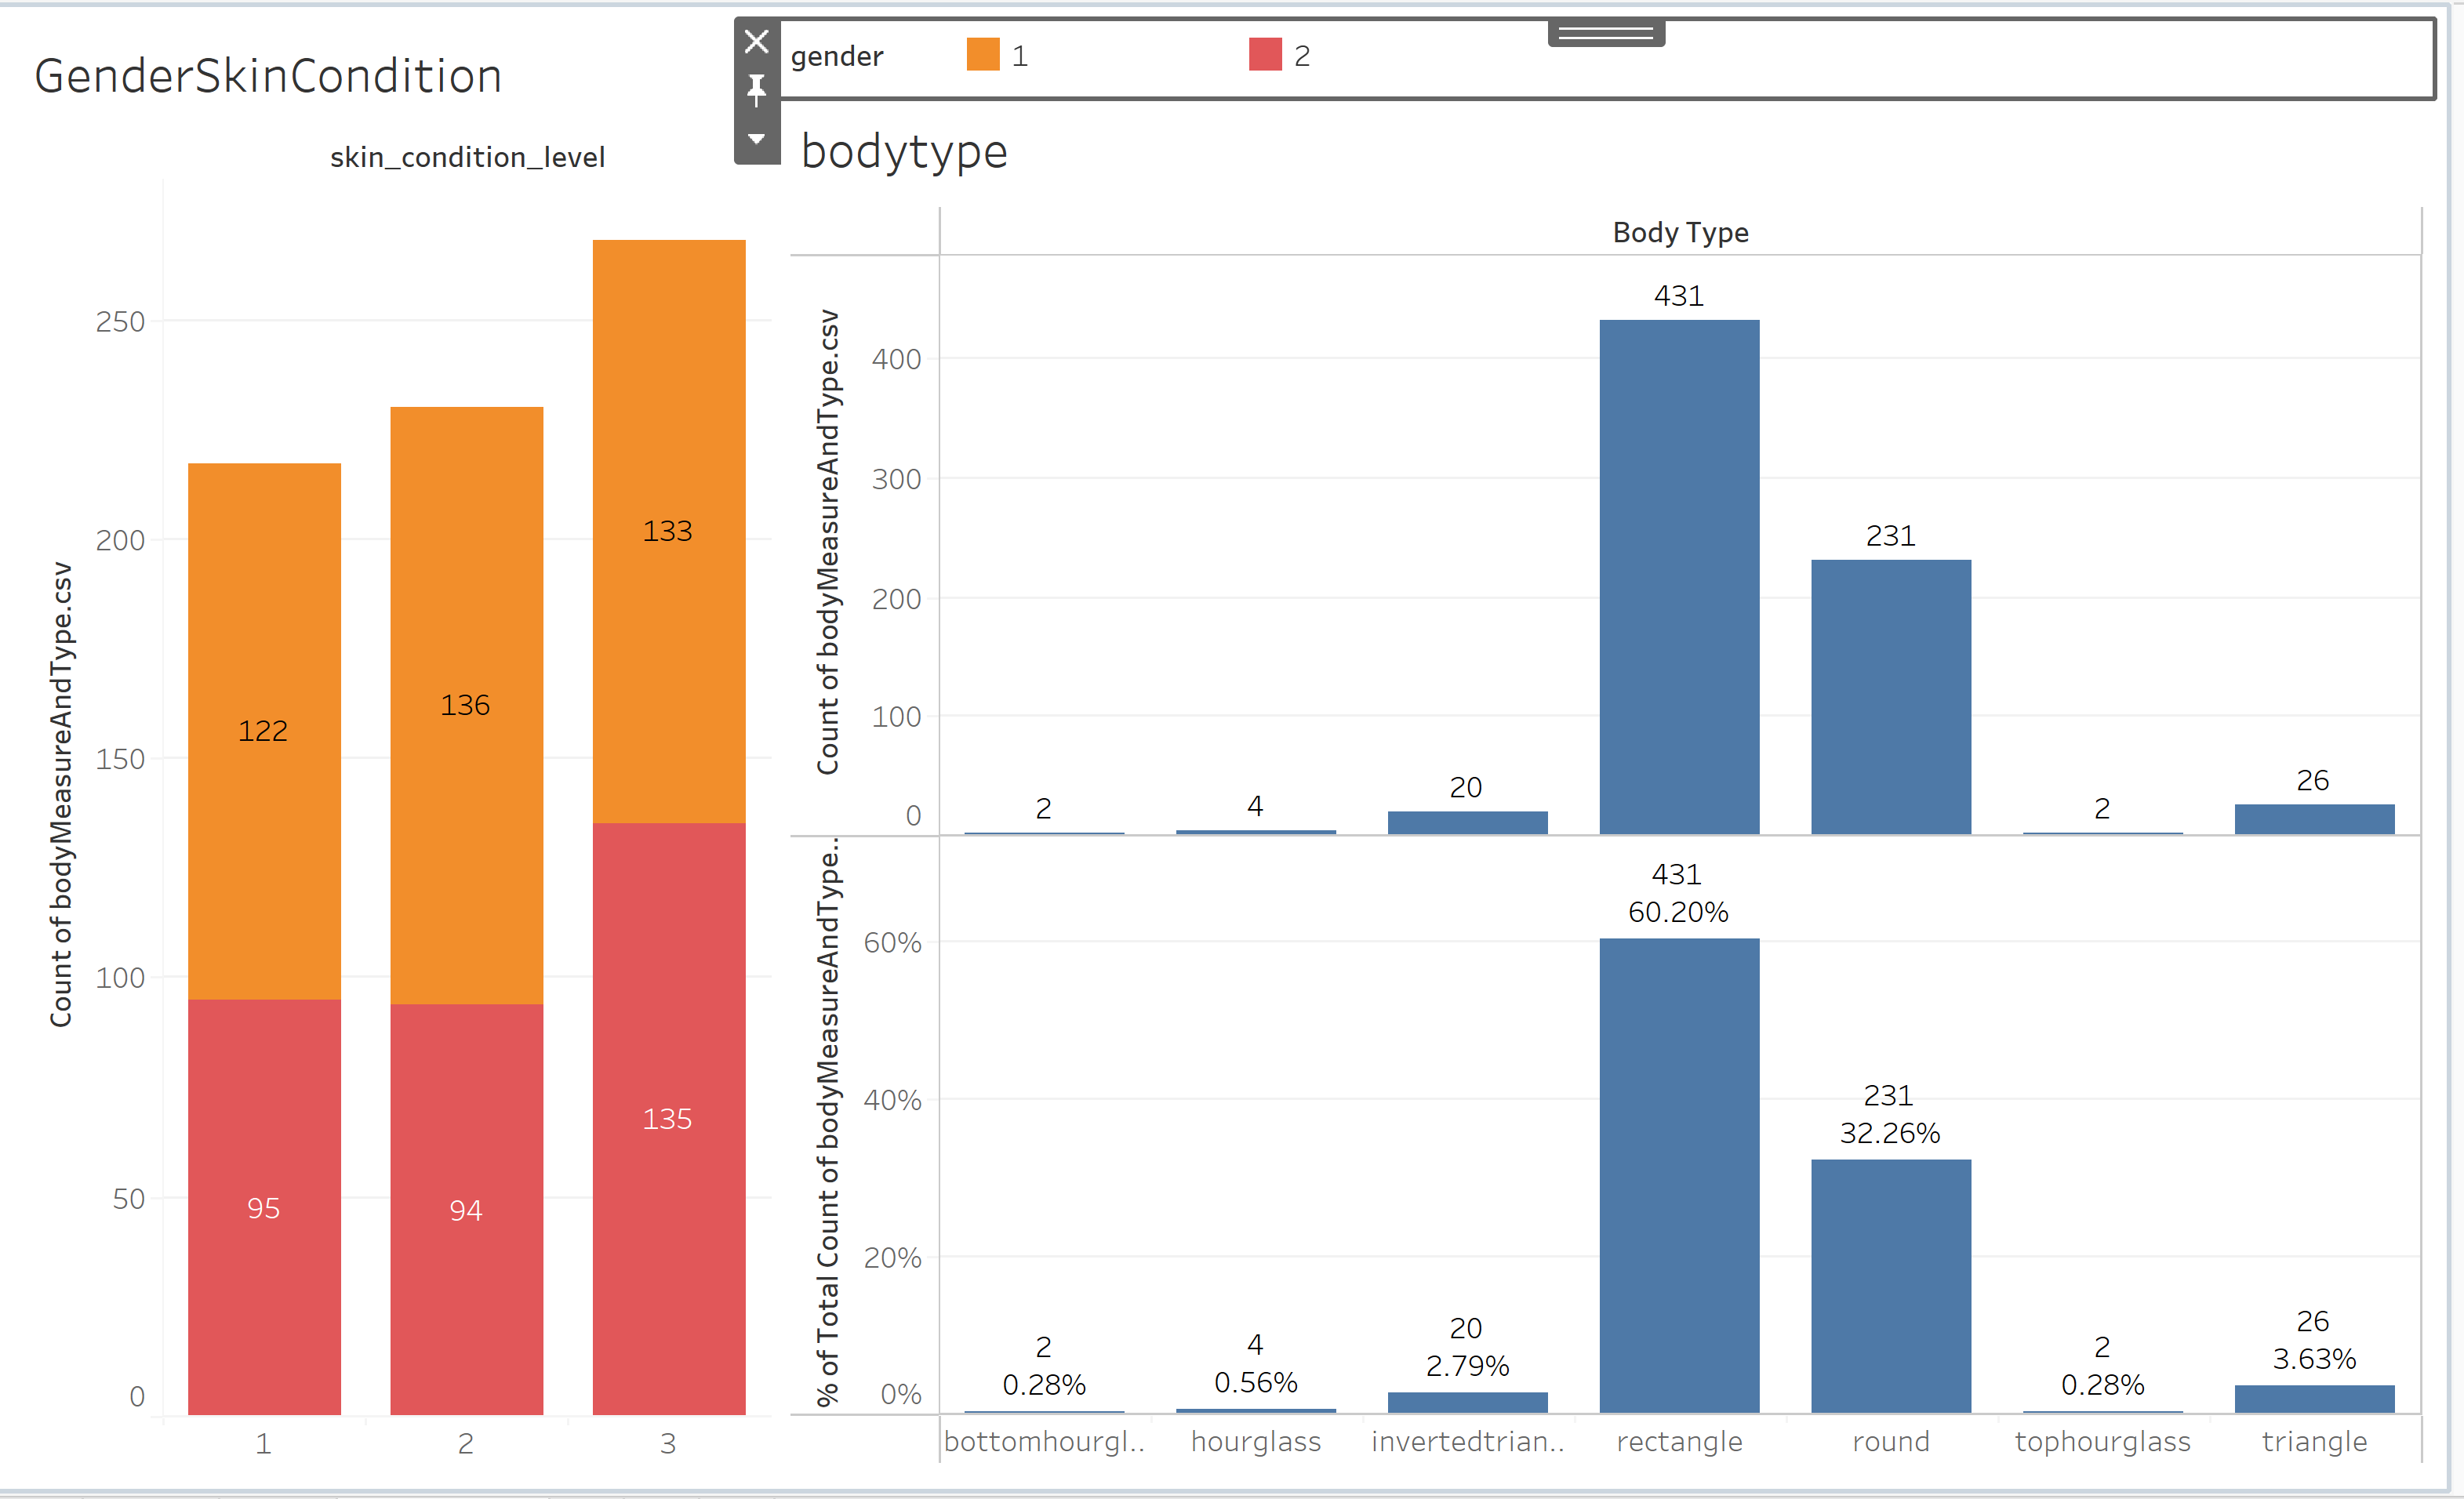
\includegraphics[scale=0.2]{images/skin.png}
\newline \centering{ {Fig. 6:} {\href{https://github.com/DecipherData/data225semproj/blob/main/Screenshots/skin.png}{Figure 6}}}\\
\justifying{The above right graph shows the distribution of body shapes in our customer database.Most of the customers are of type rectangle followed by round, hourglass customers are the least in count.}\

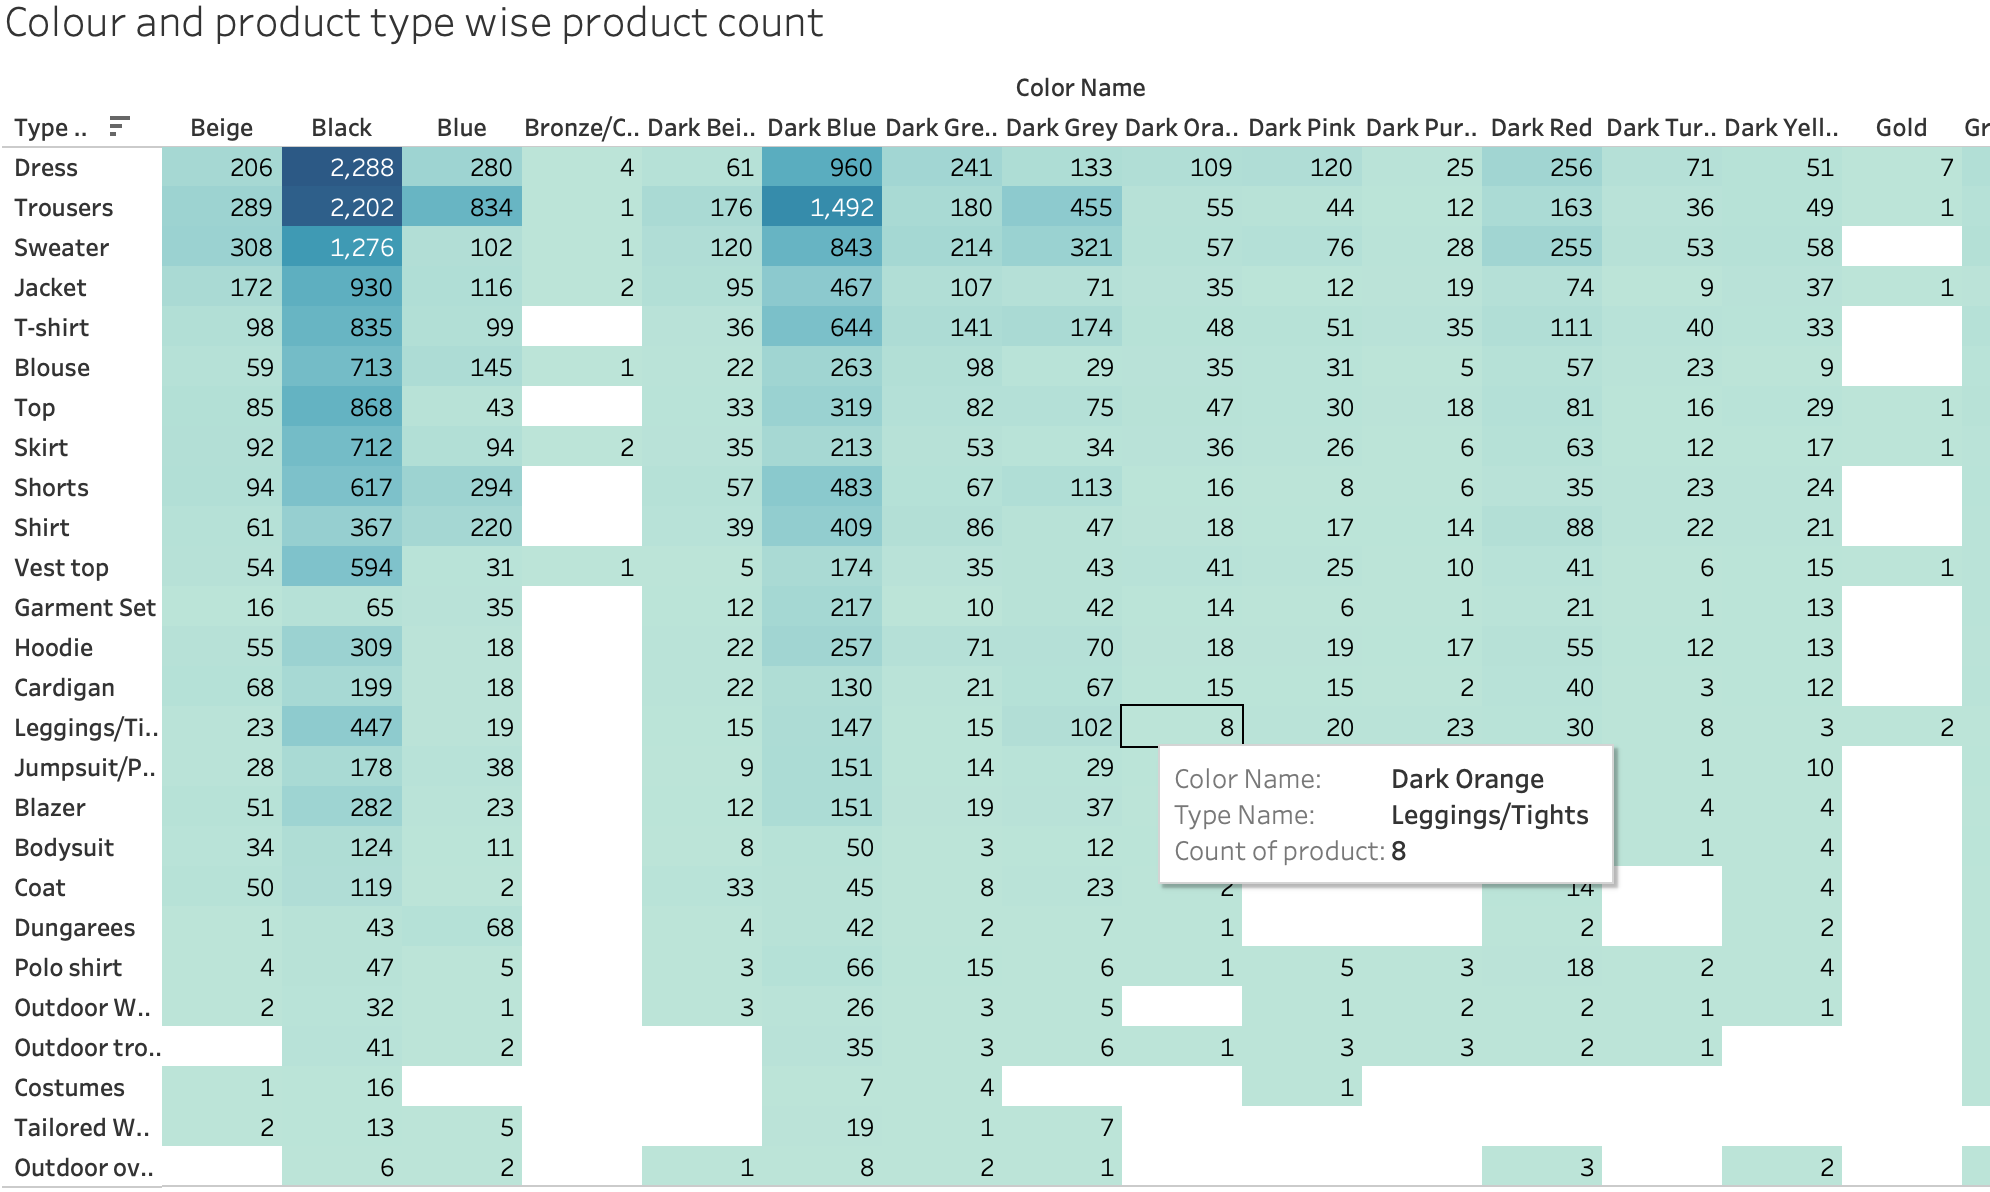
\includegraphics[scale=0.13]{images/color.png}
\newline \centering{{\href{https://github.com/DecipherData/data225semproj/blob/main/Screenshots/color.png}{Figure 7}}}\\
\justifying Following are the different analysis which we performed to get insights: 
\begin{itemize}
    \item[1.] Fabric Sales Per Year Per Month
    \item[2.] The total number of products with distinct fabrics with their quality level associated with them.
    \item[3.] Overall most sold fabric with total sales.
    \item[4.] Most sold fabric with total sales Per Year Per Month
    \item[5.] Inventory itemization based on product type, style name, fabric name, color name, count.
    \item[6.] Top 20 items in inventory based on Product Type, Product Style, Fabric Name and Color.
    \item[7.] List of names and number of product styles per body type.
    \item[8.] Count of total customers per body type and then count of customers with different skin condition levels to get a percentage of exception we are targeting for.
    \item[9.] List of Per day transaction running amount per product type for year(2020) and  List all the quarters of the years with minimum sales. To basically target quarters with more fabric options or deals for people with skin conditions.
\end{itemize}

\section{Tools and Technologies used}
\begin{itemize}
    \item[4.1] MySQL Server and MySQL workbench 
    \item[4.2] MongoDB Cluster and MongoDB Compass
    \item[4.3] Visual Studio code 
    \item[4.4] Spyder 
    \item[4.5] WinMerge 
    \item[4.6] SourceTree 
    \item[4.7] AWS Redshift 
    \item[4.8] AWS GLUE 
    \item[4.9] AWS Sagemaker 
    \item[4.10] Tableau  
    \item[4.11] Latex  
    \item[4.12] Grammarly 
    \item[4.13] Wordpress for blog  
    \item[4.14] MS Power Point Presentation  
    \item[4.15] Draw.io  
\end{itemize}

\section{Significance to the real world}\

In the present day scenario, online shopping is like breathing. Though, there are services for customization in fashion industry, major part of the trend and available services are stereotyped on measurements. Our perspective on selecting a product in this industry is not only focusing on making customization part of regular trend but also on medical conditions of skin and thus handling a part of exception cube. Not everyone knows about styling and hiring a fashion designer may cost a lot of money to the customer. This can be avoided if they are given the options that suit their body shapes in a better fashion. \

There are a fraction of customers who suffer from skin related diseases such as rash,eczema and their condition gets aggravated because of the poor quality of the fabric.Customer may not pay minute attention to fabric composition every time he or she shops. Giving them the option to select clothes based on their severity of skin condition may significantly relieve them from the external pain. \

Further, this may be beneficial for the companies as well because they will have better understanding of their customers and will stock their inventory accordingly.In addition, the amount of money spent on logistic distribution when the items are returned often may be reduced. 

\section{Lessons Learned}
\begin{itemize}
    \item[6.1] How data can be taken from different sources and extracted, Cleaned and merged according to the problem at hand.
    \item[6.2] Using the python connectivity with the MySQL server for generating functions and querying to determine an individual's body type and providing them with their desired product choices along with informing them regarding the fabric of the product and what all skin conditions is it suitable for.
    \item[6.3] Data cleaning in Spyder using python. 
    \item[6.4] Using MongoDB for fetching the body measurement composition. 
    \item[6.5] Using AWS cloud services such as AWS Redshift for data warehousing, AWS S3 for data storage, AWS Glue for our ETL process. 
    \item[6.6] Connecting AWS Redshift with Tableau for visualizing our results. 
    \item[6.7] We learned how to collaborate with each other, brainstorm and contribute in a timely manner. 
\end{itemize}

\section{Technical Difficulties and Resolutions}
\begin{itemize}
    \item[7.1] How data can be taken from different sources and extracted, cleaned and merged according to the problem at hand.
    \begin{itemize}
        \item Fabric 
        \item Skin conditions
        \item Customers
    \end{itemize}
    \item[7.2] Thus linking our synthetic data with the available data such as products was challenging.
\end{itemize}

\section{Teamwork}\ 

Right from idea sharing and conceptualization stage of this project, every member of our team played their role. We used JIRA for our tracking and agile workflow. We voluntarily picked up our own and helped each other wherever it is needed. By following agile scrum methodology, we also balanced our work correspondingly. Even though our project resembles an iterative architectural workflow there is weekly cadence to let others in team know about what is going on present task and thus leading to group discussion and evolution on our approach down the lane.
\textit{Role \& Responsibilities:}
\begin{itemize}
    \item \textbf{Vidushi Bhati} - Data Modelling, Data cleaning, Python programming, Data loading, and Data Analysis. 
    \item \textbf{Harsimran Kaur} - Data Cleaning, Data Analysis, Data visualizations and dashboard reporting, ETL.
    \item \textbf{Karnik Kalani} - Data Visualization and dashboard reporting, Data modelling.
    \item \textbf{Mounica Ayalasomayajula} - Data modelling, Data Analysis, Documentation in Latex, and PowerPoint.
    \item \textbf{Saumya Sinha} - Data cleaning and AWS Redshift, PowerPoint, and Data Analysis.
\end{itemize}
\section{Pair programming}\ 

We have collaborated extensively through Zoom, WhatsApp ,and in person for working together through the making of the project. Most of our SQL related work is directly done on AWS Redshift cluster with saved and shared Queries. For programming where we need to work with data modification and logic we used \textbf{Codeshare}(\href{https://codeshare.io/3Azd7v}{Python Code} and \href{https://codeshare.io/dwN1PM}{SQL Code} along with google docs.

\section{Agile/Scrum}
\begin{itemize}
    \item[10.1] zoom links
    \begin{itemize}
        \item \href{https://sjsu.zoom.us/j/89341269589?pwd=eGF5c1FSdzZNMjN2d1o3NmM4VWZsZz09}{Meeting 1}
        \item \href{https://sjsu.zoom.us/j/81816549366?pwd=alFvdDJDb1M4QUlONGRadG43ZHIzdz09}{Meeting 2}
        \item \href{https://sjsu.zoom.us/j/82071883934?pwd=dzc5Q0lPUFAvWWlvTitRL1NXNEljQT09}{Meeting 3}
        \item \href{https://sjsu.zoom.us/j/89073358102?pwd=N1Q1V3NjV2JaWVBwYnEvSXVWbVVtdz09}{Meeting 4}
        \item \href{https://sjsu.zoom.us/j/87444250053?pwd=eEV5UUs0UGRYell2VkVIeE5aL0FPUT09}{Meeting 5}
    \end{itemize}
    \item[10.2] Jamboard
    \begin{itemize}
        \item Link: \href{https://jamboard.google.com/d/1tzFwo7YGP86Y_Ly8sz05kr6Hp795oHY9Qj919PjHjvs/viewer}{"Click Here"}
    \end{itemize}
    \item[10.2] JIRA
    \newline Used JIRA to coordinate and distribute tasks among ourselves:
    \begin{itemize}
        \item Link: \href{https://dbms-project-group6.atlassian.net/jira/software/projects/HDPG/boards/1/roadmap}{"Click Here"}
    \end{itemize}
\end{itemize}
\section{Future Enhancements}
We can further implement some features like:
\begin{itemize}
    \item[11.1] Find solutions for analyzing needs for an efficient amount of supply according to customer’s demand and thus, minimizing the excessive unnecessary product stocks. 
    \item[11.2] The background about the customer’s choice of styles and what majority of age group people like to wear could also be determined.
    \item[11.3] Better inferences by using other advanced tools and techniques.
    \item[11.4] Alert emails or notifications once the desired product is in stock. 
    \item[11.5] This data-set will allow us to do a thorough analysis on user's behavior such as search history, click tracking and order history.
    \item[11.6] Additionally we can also draw inferences from trends based on holidays, seasons and festivals.
\end{itemize}
All of these insights can help us recommend products best suited to a customer's preferences and hence drive sales up.
\section{Conclusions}
\begin{itemize}
    \item[12.1] This project covers all the basic features of any online shopping website.  
    \item[12.2] This project is to help the customers by showing only those products which are meant for and are required by the customers based on their skin conditions and body type.
    \item[12.3] Filters provided to the customers give easy accessibility to get desired product along with fabric information.
    \item[12.4] Fulfilled our objective of learning RDBMS, Data warehouse, MySQL, ETL processes and implementing queries to create useful information and present them with the use of Data Visualization techniques.  
\end{itemize}
 \begin{thebibliography}{1}
 \bibitem{}
 2022. [Online]. Available: 
 \url{https://https://www.masterclass.com/articles/28-types-of-fabrics-and-their-uses28-different-types-of-fabric}. [Accessed: 20- April- 2022].
  \bibitem{}
 "The 12 Different Types of Fabric - Pico Cleaners | Blog", Pico Cleaners, 2022. [Online]. Available: \url{https://https://www.masterclass.com/articles/28-types-of-fabrics-and-their-uses28-different-types-of-fabric}. [Accessed: 01- May- 2022].
 \bibitem{}
 "Types of Fabrics", AanyaLinen, 2022. [Online]. Available: 
 \url{ https://www.aanyalinen.com/blogs/aanya-blog/types-of-fabrics}. [Accessed: 20- April- 2022].
 \bibitem{}
 "Types Of Fabrics | Everything You Need To Know | Sewing 101", Sewing.com, 2022. [Online]. Available: 
 \url{ https://sewing.com/fabric-types-everything-you-need-to-know/}. [Accessed: 01- May- 2022]. 
 \bibitem{}
 2022. [Online]. Available:
 \url{https://www.kaggle.com/odins0n/hm256x256}. [Accessed: 25- April- 2022].
 \bibitem{}
 "Apple Body Shape: A Comprehensive Guide | the concept wardrobe", Theconceptwardrobe.com, 2022. [Online]. Available:
 \url{https://theconceptwardrobe.com/build-a-wardrobe/apple-body-shape.}. [Accessed: 02- May- 2022].
 \bibitem{}
 "Figma", Figma, 2022. [Online]. Available:
 \url{https://www.figma.com/file.}. [Accessed: 20- April- 2022].
 \bibitem{}
 Latex-project.org, 2022. [Online]. Available:
 \url{https://www.figma.com/file.}. [Accessed: 15- April- 2022].
 \end{thebibliography}
\appendix
\renewcommand{\arraystretch}{1}
\begin{tabular}{ c  p{13cm}}  \hline
\textbf{Criteria} & \textbf{Comments} \\ \hline  
Data Sourcing and modelling & Initial ER Diagram created in Draw.io(Link: \url{https://github.com/DecipherData/data225semproj/tree/main/ER_Diagram}) Data-set is taken from Kaggle (Link: \url{https://www.kaggle.com/odins0n/hm256x256}) and Workflow is created using Figma (Link: \url{https://www.figma.com/file/vkN2Izsru0cgBYK5vJSb5x/Workflow_H%26M?node-id=0%3A1}) \\ \hline
SQL Queries & Analytical SQL Queries executed in AWS Redshift (Link: \url{https://github.com/DecipherData/data225semproj/tree/main/Queries})\\ \hline
Python Code & Python code in VSCode(Link: \url{https://codeshare.io/3Azd7v} \\ \hline
ETL & ETL performed using AWS Glue. Complete documentation is available under this location.(Link: \url{https://github.com/DecipherData/data225semproj/blob/main/ETL%20Process/ETL%20Process.docx}) \\ \hline 
Data Warehouse & AWS Redshift is used and files were stored in S3 Bucket. The evidence exist under this same ETL File(Link: \url{https://github.com/DecipherData/data225semproj/blob/main/ETL%20Process/ETL%20Process.docx}) \\ \hline 
Visualizations & Tableau was used for visualizations purposes.(Link: \url{https://github.com/DecipherData/data225semproj/tree/main/Visualization}) \\ \hline
Agile & For Agile methodology, JIRA was used{Link: \url{https://github.com/DecipherData/data225semproj/tree/main/Visualization}}\\ \hline
Team Collaboration & Jamboard is used for team collaboration(Link: \url{https://jamboard.google.com/d/1tzFwo7YGP86Y_Ly8sz05kr6Hp795oHY9Qj919PjHjvs/viewer?ts=6259b41d})\\ \hline
Documentation & Latex is used to create this report in Overleaf platform(Link: \url{https://github.com/DecipherData/data225semproj/blob/main/Report/main.tex}) \\ \hline
Version Control & Reports, Code, Screenshots, Workflow, ER Diagram (Link: \url{https://github.com/DecipherData/data225semproj})\\ \hline
ScreenShots &  All the screenshots are available in GitHub(Link: \url{https://github.com/DecipherData/data225semproj/tree/main/Screenshots})\\ \hline
\end{tabular}
\end{document}